\section{Transformada \texorpdfstring{$ \mathcal{Z} $}{Z} inversa}

\begin{frame}{Introdução}
\begin{block}{Métodos}
\begin{itemize}
	\item Dada uma função geratriz $X(z)$, como obter a \textbf{sequência de números} $x(0), x(1), x(2), ...$ que ela codifica?
	\item \textbf{Métodos} para determinar a transformada $\mathcal{Z}$ inversa:
	    \begin{enumerate}
        \item Divisão polinomial (divisão longa);
        \item Equação de diferenças;
        \item Fórmula de inversão;
        \item Frações parciais.
        \end{enumerate}
\end{itemize}
\end{block}
\end{frame}

\begin{frame}{Divisão polinomial (divisão longa)}
\begin{block}{Introdução}
\begin{itemize}
	\item A divisão polinomial ou divisão longa consiste em dividir o polinômio do numerador de $X(z)$ pelo denominador.
	\item Transformada $\mathcal{Z}$ unilateral:
\end{itemize}
$$X(z) = \sum_{k=0}^{\infty}x[k]z^{-k} = x[0] + x[1]z^{-1} + x[2]z^{-2} + \cdots $$
\end{block}
\end{frame}

\begin{frame}{Divisão polinomial (divisão longa) - Exemplo \#01}
\begin{block}{Problema}
	\[ X(z)=\dfrac{10z+5}{
		\left(z-1\right)
		\left(z-\num{0.2}\right)} \]
\end{block}
\end{frame}

\begin{frame}{Divisão polinomial (divisão longa) - Exemplo \#01}
\begin{block}{Resolução}
\begin{itemize}
    \item O primeiro passo é escrever o denominador como um polinômio, isto é:
\end{itemize}
	\[X(z)=\dfrac{10z+5}{z^2-\num{1.2}z+\num{0.2}}\]
	
\begin{itemize}
    \item Dividindo o polinômio do numerador de $X(z)$ pelo denominador, temos:
\end{itemize}

	\[ \begin{array}{r@{} r@{} r@{} r r}
		10z &{} + 5\Ph &{} &		 \multicolumn{2}{|l}{ z^{2}-\num{1,2}z+\num{0,2}} \\\cline{4-5}
		-(10z &{}-12 &{}+\hphantom{2}2\hphantom{\num[add-integer-zero=false]{.4}}z^{-1})	& \multicolumn{2}{l}{\quad10z^{-1}+17z^{-2}+\cdots}\rule{0pt}{2.6ex}\\
		\cmidrule{1-3}
		&{}17 &{}-\hphantom{2}2\hphantom{\num[add-integer-zero=false]{.4}}z^{-1}\Ph \\
		&-(17&{}-\num{20.4}z^{-1}\Ph	&{}+\num{3,4}z^{-2}) \\
		\cmidrule{2-4}
		& 			&\num{18,4}z^{-1}\Ph	&{}-\num{3,4}z^{-2}\Ph \\ & & \vdots
		\end{array} \]
\end{block}
\end{frame}

\begin{frame}{Divisão polinomial (divisão longa) - Exemplo \#01}
\begin{block}{Resolução}
\begin{itemize}
    \item Assim, a divisão longa fornece o resultado:
\end{itemize}
\[X(z)=\dfrac{10z+5}{z^2-\num{1.2}z+\num{0.2}} = 10z^{-1}+17z^{-2}+\cdots\]
\begin{itemize}
    \item Comparando com o somatório da transformada $\mathcal{Z}$ unilateral, temos: 
\end{itemize}

$$\bm{x[0] = 0, \quad x[1] = 10, \quad x[2] = 17, \quad \cdots}$$
\begin{itemize}
    \item $x[k]$ é dado por uma sequência de números (sinal no domínio de amostras). A divisão sucessiva poderia ter continuada para obter as próximas amostras.
    \item O procedimento é simples, mas normalmente \textbf{não fornece uma expressão fechada} para a transformada inversa.
\end{itemize}
\end{block}
\end{frame}

\begin{frame}{Equação de diferenças}
\begin{block}{Introdução}
\begin{itemize}
	\item A fim de usar uma \textbf{equação de diferença} para  obter a transformada $\mathcal{Z}$ inversa de uma função $X(z)$, imaginamos que essa função corresponde à transformada $\mathcal{Z}$ de um sinal $x(k)$, que é a resposta de um sistema a uma entrada $u[k]$ \textbf{impulsiva unitária}. 
	\item Como, nesse caso, $U(z) = 1$, temos que
\end{itemize}
$$\boxed{x[k] = \mathcal{Z}^{-1} \left\lbrace X(z)U(z) \right\rbrace}$$
\begin{itemize}
	\item Duas \textbf{condições} são necessárias para a utilização deste  método: 
	\begin{enumerate}
	    \item A entrada deve ser um impulso unitário.
	    \item As condições iniciais devem ser nulas.
	\end{enumerate}
\end{itemize}
\end{block}
\end{frame}

\begin{frame}{Equação de diferenças - Exemplo \#01}
\begin{block}{Problema}
	\[ X(z)=\dfrac{10z+5}{
		\left(z-1\right)
		\left(z-\num{0.2}\right)} \]
\end{block}
\end{frame}

\begin{frame}{Equação de diferenças - Exemplo \#01}
\begin{block}{Resolução}
\begin{itemize}
    \item O primeiro passo é escrever o denominador como um polinômio, isto é:
\end{itemize}
	\[X(z)=\dfrac{10z+5}{z^2-\num{1.2}z+\num{0.2}}\]
\begin{itemize}
    \item Usando a definição anterior, temos que
\end{itemize}
    \[X(z)=\dfrac{10z+5}{z^2-\num{1.2}z+\num{0.2}} \ U(z)\] 
\begin{itemize}
    \item Multiplicando cruzado, vem:
\end{itemize}
    \[X(z)\left(z^2-\num{1.2}z+\num{0.2}\right) = \left(10z+5\right)U(z)\]
    \[X(z)\left(1-\num{1.2}z^{-1}+\num{0.2}z^{-2}\right) = \left(10z^{-1}+5z^{-2}\right)U(z)\]
\end{block}
\end{frame}

\begin{frame}{Equação de diferenças - Exemplo \#01}
\begin{block}{Resolução}
\begin{itemize}
    \item Tomando a transformada $\mathcal{Z}$ inversa, temos:
\end{itemize}
	\[x[k]-\num{1.2}x[k-1]+\num{0.2}x[k-2]=10u[k-1]+5u[k-2]\]
	\[x[k]=\num{1.2}x[k-1]-\num{0.2}x[k-2]+10u[k-1]+5u[k-2]\]
\begin{itemize}
    \item Basta agora resolver essa equação considerando $u[k] = \delta[k]$ com \textbf{condições iniciais nulas}. Sendo assim, $u[0] = 1$ e $x[-1] = x[-2] = 0$. 
\end{itemize}

    $$x[0] = \num{1.2}x[-1] - \num{0.2}x[-2] + 10u[-1] + 5u[-2] = \bm{0}$$
    $$x[1] = \num{1.2}x[0] - \num{0.2}x[-1] + 10u[0] + 5u[-1] = \bm{10}$$   
    $$x[2] = \num{1.2}x[1] - \num{0.2}x[0] + 10u[1] + 5u[0] = \bm{17}$$

\begin{itemize}
    \item Esta solução \textbf{coincide} com a solução encontrada no primeiro método.
\end{itemize}
\end{block}
\end{frame}

\begin{frame}{Fórmula de inversão}
\begin{block}{Introdução}
\begin{itemize}
	\item A transformada $\mathcal{Z}$ inversa de uma função $X(z)$ pode ser calculada pela integral de linha
\end{itemize}

	\[ x[k]=\dfrac{1}{2\pi j}\oint_{\Gamma} X(z)z^{k-1}\dif z, \]

onde $\Gamma$ é um caminho fechado que inclui todos os polos finitos de $X(z)z^{k-1}$.

\begin{itemize}
	\item Mesma dificuldade da transformada inversa de Laplace.
	\item Cauchy introduz uma solução mais simples para resolver a integral:
\end{itemize}
$$x[k] = \sum_{\text{pol}\left[X(z)z^{k-1}\right]}^{} \text{res}\left[X(z)z^{k-1}\right]$$

em que em que pol[.] e res[.] indicam os polos e  os respectivos resíduos das funções nos argumentos.
\end{block}
\end{frame}

\begin{frame}{Fórmula de inversão - Exemplo \#01}
\begin{block}{Problema}
	\[ X(z)=\dfrac{10z+5}{
		\left(z-1\right)
		\left(z-\num{0.2}\right)} \]
\end{block}
\end{frame}

\begin{frame}{Fórmula de inversão - Exemplo \#01}
\begin{block}{Resolução}
\begin{itemize}
    \item Calculando os resíduos de $X(z)z^{k-1}$, temos:
\end{itemize}
\begin{align*}
r_1&=\eval{X(z)z^{k-1}\left(z-1\right)}_{z=1}= \\
&= \eval{\dfrac{10z+5}{z-\num{0.2}} \ z^{k-1}}_{z=1}= \\
&= \dfrac{10+5}{1-\num{0.2}} \ (1)^{k-1} = \num{18.75}
\end{align*}
\end{block}
\end{frame}

\begin{frame}{Fórmula de inversão - Exemplo \#01}
\begin{block}{Resolução}
\begin{align*}
r_2 &=\eval{X(z)z^{k-1}\left(z-\num{0.2}\right)}_{z=\num{0.2}}= \\
&= \eval{\dfrac{10z+5}{z-1} \ z^{k-1}}_{z=\num{0.2}}= \\
&= \dfrac{2+5}{\num{0.2}-1} \ (\num{0.2})^{k-1} = -\num{43.75} \ (\num{0.2})^k
\end{align*}
\end{block}
\end{frame}

\begin{frame}{Fórmula de inversão - Exemplo \#01}
\begin{block}{Resolução}
\begin{itemize}
    \item Note que para $k = 0$, $X(z)z^{k-1}$ torna-se $X(z)/z$, que  tem um polo a mais ($z = 0$). Deste modo, para $k = 0$ haverá um resíduo a mais, que é:
\end{itemize}
\begin{align*}
r_0 &=\eval{\dfrac{10z+5}{\left(z-1\right)\left(z-\num{0.2}\right)z} \ z}_{z=0}= \\
&= \eval{\dfrac{10z+5}{\left(z-1\right)\left(z-\num{0.2}\right)}}_{z=0} = \\
&= \dfrac{5}{(-1)(-\num{0.2})}=25
\end{align*}
\end{block}
\end{frame}

\begin{frame}{Fórmula de inversão - Exemplo \#01}
\begin{block}{Resolução}
\begin{itemize}
    \item Logo, a transformada $\mathcal{Z}$ inversa é dada por:
\end{itemize}

$$k = 0 \implies x[k] = r_0 + r_1 + r_2 = \bm{0}$$

\begin{align*}
k \geq 1 \implies & x[k] = r_1 + r_2 = \num{18.75} -\num{43.75} \ (\num{0.2})^k \\
& x[1] = \num{18.75} -\num{43.75} \ (\num{0.2})^1 = \bm{10} \\
& x[2] = \num{18.75} -\num{43.75} \ (\num{0.2})^2 = \bm{17}
\end{align*}
\begin{itemize}
    \item Esta solução \textbf{coincide} com as outras duas soluções anteriores.
\end{itemize}
\end{block}
\end{frame}

\begin{frame}{Frações parciais}
\begin{block}{Introdução}
\begin{itemize}
    \item Representa uma das maneiras mais práticas de fazer a transformada $\mathcal{Z}$ inversa. 
    \item Além disso, o resultado  normalmente apresentará uma \textbf{forma fechada}.
	\item Consiste na divisão de polinômios em \textbf{potências negativas de} \bm{$z$}, geralmente notado em sistemas LTI discretos.
\end{itemize}
	
$$X(z) = \dfrac{B(z)}{A(z)} = \dfrac{b_{m}z^{m}+b_{m-1}z^{m-1}+\cdots+b_{1}z+b_{0}}{a_{n}z^{n}+a_{n-1}z^{n-1}+\cdots+a_{1}z+a_{0}}, \bm{m < n}, a_n \neq 0$$
	
\textbf{Obs.:} Caso não esteja nesta forma, basta dividir pela maior potência de $ z $.

\begin{itemize}
    \item \textbf{Objetivo:} escrever $ X(z) $ como uma \textbf{soma de frações parciais}:
\end{itemize}
	\[ X(z)=\sum_{i=1}^{n}\dfrac{A_i}{1-d_iz^{-1}} \, , \text{ expansão em termos de \textbf{primeira ordem}} \]
\end{block}
\end{frame}

\begin{frame}{Frações parciais}
\begin{block}{Ambiguidade}
	Lembre-se da \textbf{ambiguidade} existente no domínio $ z $, a não ser que a ROC seja dada.
	\begin{align*}
	A_i(d_i)^{k}u[k]&\overset{\mathcal{Z}}{\Longleftrightarrow}\dfrac{A_i}{1-d_iz^{-1}}& \, &\text{ROC }|z|>|d_i|\, ,\text{ direito (\textbf{causal})}\\
	-A_i(d_i)^{k}u[-k-1]&\overset{\mathcal{Z}}{\Longleftrightarrow}\dfrac{A_i}{1-d_iz^{-1}}& \, &\text{ROC }|z|<|d_i|\, ,\text{ esquerdo (\textbf{não causal})}
	\end{align*}
	
	\begin{itemize}
		\item Quando a ROC de $ X(z) $ possui raio \textbf{maior} que o polo de um dado termo: \textit{right-sided}.
		\item Quando a ROC de $ X(z) $ possui o raio \textbf{menor} que o polo de um dado termo: \textit{left-sided}.
	\end{itemize}
\end{block}
\end{frame}

\begin{frame}{Frações parciais - Exemplo \#01}
\begin{block}{Problema}
	\[ X(z)=\dfrac{10z+5}{
		\left(z-1\right)
		\left(z-\num{0.2}\right)} \]
		
	Dado: sistema causal
\end{block}
\end{frame}

\begin{frame}{Frações parciais - Exemplo \#01}
	\begin{block}{Resolução}
	    \[ X(z)=\dfrac{10z^{-1}+5z^{-2}}{(1-z^{-1})(1-\num{0.2}z^{-1})} \quad m=n=2\quad \text{\xmark} \]
	    
		\vspace{0.5cm}
		
		\[ \begin{array}{r r}
	5z^{-2}+10z^{-1} & \multicolumn{1}{|c}{\num{0,2}z^{-2}-\num{1,2}z^{-1}+1}\\\cline{2-2}
	-(5z^{-2}-30z^{-1}+25)	&25\rule{0pt}{2.6ex}\\
	\cmidrule{1-1}
	40z^{-1}-25
	\end{array} \]		
	
\end{block}
\end{frame}

\begin{frame}{Frações parciais - Exemplo \#01}
\begin{block}{Resolução}
	\begin{align*}
	X(z)&=25+\dfrac{40z^{-1}-25}{(1-z^{-1})(1-\num{0.2}z^{-1})}\\
	X(z)&=\dfrac{A}{1-z^{-1}}+\dfrac{B}{1-\num{0,2}z^{-1}}=\dfrac{40z^{-1}-25}{(1-z^{-1})(1-\num{0,2}z^{-1})}
	\end{align*}
\end{block}
\end{frame}

\begin{frame}{Frações parciais - Exemplo \#01}
\begin{block}{Resolução}
	\begin{align*}
	A&=\eval{X(z)\left(1-z^{-1}\right)}_{z^{-1}=1}=\\
	&=\eval{\dfrac{40z^{-1}-25}{1-\num{0.2}z^{-1}}}_{z^{-1}=1}=\\
	&=\dfrac{40-25}{1-\num{0.2}}=\num{18.75}
	\end{align*}
\end{block}
\end{frame}

\begin{frame}{Frações parciais - Exemplo \#01}
\begin{block}{Resolução}
	\begin{align*}
	B&=\eval{X(z)\left(1-\num{0.2}z^{-1}\right)}_{z^{-1}=5}=\\
	&=\eval{\dfrac{40z^{-1}-25}{1-z^{-1}}}_{z^{-1}=5}=\\
	&=\dfrac{200-25}{1-5}=-\num{43.75}
	\end{align*}
\end{block}
\end{frame}

\begin{frame}{Frações parciais - Exemplo \#01}
\begin{block}{Resolução}
		\[ \therefore X(z)=25+\underbrace{\dfrac{\num{18.75}}{1-z^{-1}}}_{1}-\underbrace{\dfrac{\num{43.75}}{1-\num{0.2}z^{-1}}}_{2} \]
		
		\begin{enumerate}
			\item polo @ $ z=1 \rightarrow $ \textit{right-sided} $ \leftrightarrow \num{18.75}(1)^{k}u[k] $
			\item polo @ $ z=\num{0.2} \rightarrow $ \textit{right-sided} $ \leftrightarrow -\num{43.75}(\num{0.2})^{k}u[k] $
		\end{enumerate}

Logo, $ x[k]=25\delta[k]+\num{18.75}(1)^{k}u[k]-\num{43.75}(\num{0.2})^{k}u[k] $

	\begin{align*}
	x[0] &= 25 + \num{18.75} -\num{43.75} = \bm{0} \\
	x[1] &= 0 + \num{18.75} -\num{43.75}(\num{0.2}) = \bm{10} \\
    x[2] &= 0 + \num{18.75} -\num{43.75} (\num{0.2})^2 = \bm{17} 
    \end{align*}
    
\begin{itemize}
    \item Esta solução \textbf{coincide} com as outras três soluções anteriores.
\end{itemize}
\end{block}
\end{frame}

































\begin{frame}{Frações parciais - Exemplo \#02}
\begin{block}{Problema}
	\[ X(z)=\dfrac{1-z^{-1}+z^{-2}}{
		\left( 1-\dfrac{1}{2}z^{-1} \right)
		\left( 1-2z^{-1} \right)
		\left( 1-z^{-1} \right) } \quad m<n \quad \text{\cmark} \]
	
	Dado: ROC: $ 1<|z|<2 $
\end{block}
\end{frame}


\begin{frame}{Frações parciais - Exemplo \#02}
	\begin{block}{Resolução}
		\[ X(z)=\dfrac{A}{1-\dfrac{1}{2}z^{-1}}+\dfrac{B}{1-2z^{-1}}+\dfrac{C}{1-z^{-1}}= \dfrac{1-z^{-1}+z^{-2}}{\left( 1-\dfrac{1}{2}z^{-1} \right) \left( 1-2z^{-1} \right) \left( 1-z^{-1} \right) } \]
	\end{block}
\end{frame}


\begin{frame}{Frações parciais - Exemplo \#02}
\begin{block}{Resolução}
	\begin{align*}
	A&=\eval{X(z)\left(1-\dfrac{1}{2}z^{-1}\right)}_{z^{-1}=2}=\\
	&=\eval{\dfrac{1-z^{-1}+z^{-2}}{\left(1-2z^{-1}\right)\left(1-z^{-1}\right)}}_{z^{-1}=2}=\\
	&=\dfrac{1-2+4}{(1-4)(1-2)}=1
	\end{align*}
\end{block}
\end{frame}

\begin{frame}{Frações parciais - Exemplo \#02}
\begin{block}{Resolução}
	\begin{align*}
	B&=\eval{X(z)\left(1-2z^{-1}\right)}_{z^{-1}=1/2}=\\
	&=\left. \dfrac{1-z^{-1}+z^{-2}}{\left(1-\dfrac{1}{2}z^{-1}\right)\left(1-z^{-1} \right)}\right| _{z^{-1}=1/2}=\\
	&=\dfrac{1-1/2+1/4}{(1-1/4)(1-1/2)}=2
	\end{align*}
\end{block}
\end{frame}

\begin{frame}{Frações parciais - Exemplo \#02}
\begin{block}{Resolução}
	\begin{align*}
	C&=\eval{X(z)\left(1-z^{-1}\right)}_{z^{-1}=1}=\\
	&=\left. \dfrac{1-z^{-1}+z^{-2}}{\left(1-\dfrac{1}{2}z^{-1}\right)\left(1-2z^{-1} \right)}\right| _{z^{-1}=1}=\\
	&=\dfrac{1-1+1}{(1-1/2)(1-2)}=-2
	\end{align*}
\end{block}
\end{frame}

\begin{frame}{Frações parciais - Exemplo \#02}
\begin{block}{Resolução}
	\begin{minipage}{0.45\linewidth}
		\[ \therefore X(z)=\underbrace{\dfrac{1}{1-\dfrac{1}{2}z^{-1}}}_{1}+\underbrace{\dfrac{2}{1-2z^{-1}}}_{2}-\underbrace{\dfrac{2}{1-z^{-1}}}_{3} \]
		
		\begin{enumerate}
			\item polo @ $ z=1/2 \rightarrow $ \textit{right-sided} $ \leftrightarrow \left( \dfrac{1}{2}\right) ^{k}u[k] $
			\item polo @ $ z=2 \rightarrow $ \textit{left-sided} $ \leftrightarrow -2(2)^{k}u[-k-1] $
			\item polo @ $ z=1 \rightarrow $ \textit{right-sided} $ \leftrightarrow -2u[k] $
		\end{enumerate}
	\end{minipage}
	\hfill
	\begin{minipage}{0.45\linewidth}
		\centering
		\scalebox{0.7}{

\tikzset{every picture/.style={line width=0.75pt}} %set default line width to 0.75pt        

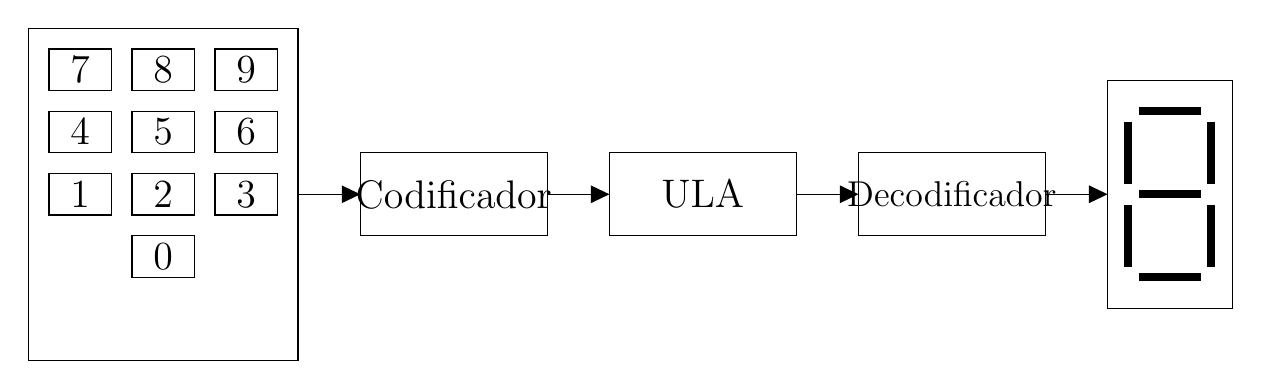
\begin{tikzpicture}[x=0.75pt,y=0.75pt,yscale=-1,xscale=1]
%uncomment if require: \path (0,300); %set diagram left start at 0, and has height of 300

%Shape: Rectangle [id:dp8798188650405219] 
\draw   (30,50) -- (160,50) -- (160,210) -- (30,210) -- cycle ;
%Shape: Rectangle [id:dp593444354888008] 
\draw   (40,60) -- (70,60) -- (70,80) -- (40,80) -- cycle ;
%Shape: Rectangle [id:dp4412846627526852] 
\draw   (80,60) -- (110,60) -- (110,80) -- (80,80) -- cycle ;
%Shape: Rectangle [id:dp2343273962035186] 
\draw   (120,60) -- (150,60) -- (150,80) -- (120,80) -- cycle ;
%Shape: Rectangle [id:dp05777918912875246] 
\draw   (40,90) -- (70,90) -- (70,110) -- (40,110) -- cycle ;
%Shape: Rectangle [id:dp9955010424516375] 
\draw   (80,90) -- (110,90) -- (110,110) -- (80,110) -- cycle ;
%Shape: Rectangle [id:dp24021539717259266] 
\draw   (120,90) -- (150,90) -- (150,110) -- (120,110) -- cycle ;
%Shape: Rectangle [id:dp36169684584711925] 
\draw   (40,120) -- (70,120) -- (70,140) -- (40,140) -- cycle ;
%Shape: Rectangle [id:dp7232437677097003] 
\draw   (80,120) -- (110,120) -- (110,140) -- (80,140) -- cycle ;
%Shape: Rectangle [id:dp6884539525496838] 
\draw   (120,120) -- (150,120) -- (150,140) -- (120,140) -- cycle ;
%Shape: Rectangle [id:dp9961423077173726] 
\draw   (80,150) -- (110,150) -- (110,170) -- (80,170) -- cycle ;
%Shape: Rectangle [id:dp6643057105712631] 
\draw   (190,110) -- (280,110) -- (280,150) -- (190,150) -- cycle ;
%Shape: Rectangle [id:dp7094011053258715] 
\draw   (550,75) -- (610,75) -- (610,185) -- (550,185) -- cycle ;
%Shape: Rectangle [id:dp2693438921699036] 
\draw   (310,110) -- (400,110) -- (400,150) -- (310,150) -- cycle ;
%Shape: Rectangle [id:dp3654960401722005] 
\draw   (430,110) -- (520,110) -- (520,150) -- (430,150) -- cycle ;
%Straight Lines [id:da6667328032348829] 
\draw    (160,130) -- (188,130) ;
\draw [shift={(190,130)}, rotate = 180] [fill={rgb, 255:red, 0; green, 0; blue, 0 }  ][line width=0.75]  [draw opacity=0] (8.93,-4.29) -- (0,0) -- (8.93,4.29) -- cycle    ;

%Straight Lines [id:da5165651690517046] 
\draw    (280,130) -- (308,130) ;
\draw [shift={(310,130)}, rotate = 180] [fill={rgb, 255:red, 0; green, 0; blue, 0 }  ][line width=0.75]  [draw opacity=0] (8.93,-4.29) -- (0,0) -- (8.93,4.29) -- cycle    ;

%Straight Lines [id:da17751850693095572] 
\draw    (400,130) -- (428,130) ;
\draw [shift={(430,130)}, rotate = 180] [fill={rgb, 255:red, 0; green, 0; blue, 0 }  ][line width=0.75]  [draw opacity=0] (8.93,-4.29) -- (0,0) -- (8.93,4.29) -- cycle    ;

%Straight Lines [id:da4998570413390182] 
\draw [color={rgb, 255:red, 0; green, 0; blue, 0 }  ,draw opacity=1 ][line width=3]    (560,95) -- (560,125) ;


%Straight Lines [id:da05287212083080073] 
\draw [color={rgb, 255:red, 0; green, 0; blue, 0 }  ,draw opacity=1 ][line width=3]    (600,95) -- (600,125) ;


%Straight Lines [id:da9146969001147236] 
\draw [color={rgb, 255:red, 0; green, 0; blue, 0 }  ,draw opacity=1 ][line width=3]    (560,135) -- (560,165) ;


%Straight Lines [id:da37610179690179124] 
\draw [color={rgb, 255:red, 0; green, 0; blue, 0 }  ,draw opacity=1 ][line width=3]    (600,135) -- (600,165) ;


%Straight Lines [id:da2798262228013664] 
\draw [color={rgb, 255:red, 0; green, 0; blue, 0 }  ,draw opacity=1 ][line width=3]    (595,130) -- (565,130) ;


%Straight Lines [id:da15184615547446478] 
\draw [color={rgb, 255:red, 0; green, 0; blue, 0 }  ,draw opacity=1 ][line width=3]    (595,90) -- (565,90) ;


%Straight Lines [id:da20609816632014244] 
\draw [color={rgb, 255:red, 0; green, 0; blue, 0 }  ,draw opacity=1 ][line width=3]    (595,170) -- (565,170) ;


%Straight Lines [id:da16937059284664002] 
\draw    (520,130) -- (548,130) ;
\draw [shift={(550,130)}, rotate = 180] [fill={rgb, 255:red, 0; green, 0; blue, 0 }  ][line width=0.75]  [draw opacity=0] (8.93,-4.29) -- (0,0) -- (8.93,4.29) -- cycle    ;


% Text Node
\draw (135,70) node   {\Large $9$};
% Text Node
\draw (95,70) node   {\Large $8$};
% Text Node
\draw (55,70) node   {\Large $7$};
% Text Node
\draw (135,100) node   {\Large $6$};
% Text Node
\draw (135,130) node   {\Large $3$};
% Text Node
\draw (95,160) node   {\Large $0$};
% Text Node
\draw (95,130) node   {\Large $2$};
% Text Node
\draw (95,100) node   {\Large $5$};
% Text Node
\draw (55,100) node   {\Large $4$};
% Text Node
\draw (55,130) node   {\Large $1$};
% Text Node
\draw (235,130) node  [align=left] {\Large Codificador};
% Text Node
\draw (355,130) node  [align=left] {\Large ULA};
% Text Node
\draw (475,130) node [scale=0.9] [align=left] {\Large Decodificador};


\end{tikzpicture}
}
	\end{minipage}
	
	Logo, $ x[k]=\left( \dfrac{1}{2}\right)^{k}u[k]-2(2)^{k}u[-k-1]-2u[k]  $
\end{block}
\end{frame}

\begin{frame}{Frações parciais - Exemplo \#03}
\begin{block}{Problema}
	\[ X(z)=\dfrac{z^{3}-10z^{2}-4z+4}{2z^{3}-2z^{2}-4z} \]
	
	Dado: ROC: $ 0<|z|<1 $
\end{block}
\end{frame}


\begin{frame}{Frações parciais - Exemplo \#03}
\begin{block}{Resolução}

    \[ X(z)=\dfrac{1-10z^{-1}-4z^{-2}+4z^{-3}}{2-2z^{-1}-4z^{-2}} \quad m=3>n=2\quad \text{\xmark} \]
    
    \vspace{0.5cm}
    
	\[ \begin{array}{r@{} r@{} r@{} r r}
	4z^{-3} &{}-4z^{-2} &{}-10z^{-1} 	&{}+1\Ph		& \multicolumn{1}{|c}{-4z^{-2}-2z^{-1}+2}\\\cline{5-5}
	-(4z^{-3} &{}+2z^{-2} &{}-2z^{-1})	&	&-z^{-1}+3/2\rule{0pt}{2.6ex}\\
	\cmidrule{1-3}
	&{}-6z^{-2} &{}-8z^{-1}\Ph	&{}+1\Ph\\
	&-(-6z^{-2}	&{}-3z^{-1}\Ph	&{}+3) \\
	\cmidrule{2-4}
	& 			&-5z^{-1}\Ph	&{}-2\Ph
	\end{array} \]
\end{block}
\end{frame}


\begin{frame}{Frações parciais - Exemplo \#03}
\begin{block}{Resolução}
	\begin{align*}
	X(z)&=-z^{-1}+3/2+\dfrac{-5z^{-1}-2}{2-2z^{-1}-4z^{-2}}\\
	X(z)&=-z^{-1}+3/2+\dfrac{-5z^{-1}-2}{2(1+z^{-1})(1-2z^{-1})}\\
	X(z)&=-z^{-1}+3/2+\dfrac{-\dfrac{5}{2}z^{-1}-1}{(1+z^{-1})(1-2z^{-1})}\\
	X(z)&=\dfrac{A}{1+z^{-1}}+\dfrac{B}{1-2z^{-1}}=\dfrac{-\dfrac{5}{2} z^{-1}-1}{(1+z^{-1})(1-2z^{-1})}
	\end{align*}
\end{block}
\end{frame}


\begin{frame}{Frações parciais - Exemplo \#03}
\begin{block}{Resolução}
	\begin{align*}
	A&=\eval{X(z)(1+z^{-1})}_{z^{-1}=-1}=\\
	 &=\eval{\dfrac{-\dfrac{5}{2}z^{-1}-1}{1-2z^{-1}}}_{z^{-1}=-1}=\\
	 &=\dfrac{5/2-1}{1+2}=1/2
	\end{align*}
\end{block}
\end{frame}


\begin{frame}{Frações parciais - Exemplo \#03}
\begin{block}{Resolução}
	\begin{align*}
	B&=\eval{X(z)(1-2z^{-1})}_{z^{-1}=1/2}=\\
	 &=\eval{\dfrac{-\dfrac{5}{2}z^{-1}-1}{1+z^{-1}}}_{z^{-1}=1/2}=\\
	 &=\dfrac{-5/4-1}{1+1/2}=-3/2
	\end{align*}
\end{block}
\end{frame}


\begin{frame}{Frações parciais - Exemplo \#03}
\begin{block}{Resolução}
	\begin{minipage}{0.45\linewidth}
		\[ \therefore X(z)=-z^{-1}+3/2+\underbrace{\dfrac{1/2}{1+z^{-1}}}_{1}-\underbrace{\dfrac{3/2}{1-2z^{-1}}}_{2} \]
		
		\begin{enumerate}
			\item polo @ $ z=-1 \overset{|z|<1}{\longrightarrow} $ \textit{left-sided} $ \rightarrow -\dfrac{1}{2}(-1)^{k}u[-k-1] $
			\item polo @ $ z=2 \rightarrow $ \textit{left-sided} $ \rightarrow \dfrac{3}{2}(2)^{k}u[-k-1] $
		\end{enumerate}
	\end{minipage}
	\hfill
	\begin{minipage}{0.45\linewidth}
		\centering
		\scalebox{0.7}{\deftkzbds
	
\begin{tikzpicture}[auto, node distance=2cm,>=Latex]
	
	\node [input, name=input] {};
	
	\node [coordinate, right=of input] (junction) {};
	\draw (input) -- node[near start] {$E(z)$} (junction);
	
	\node [block, right=of junction] (ei) {$ C_i(z) $};
	\node [block, above=of ei] (kp) {$ C_p(z) $};
	\node [block, below=of ei] (cd) {$ C_d(z) $};
	
	\draw [->] (junction) -- (ei);
	\draw [->] (junction) |- (kp);
	\draw [->] (junction) |- (cd);
	
	\node [sum, right=2cm of ei] (sum) {$ \phantom{\sum} $};
	\draw (sum) ++(-8pt,-8pt) -- ++(16pt,16pt) ++(-16pt,0pt) -- +(16pt,-16pt);
	
	\draw [<-] (sum) -- node[very near start, above] {$ + $} (ei);
	\draw [<-] (sum) |- node[very near start, right] {$ + $} (kp);
	\draw [<-] (sum) |- node[very near start, left] {$ + $} (cd);
	
	\node [output, right=of sum] (output) {};
	\draw [->] (sum) -- node[near end] {$ U(z) $} (output);
\end{tikzpicture}}
	\end{minipage}
	
	Logo, $ x[k]=-\delta[k-1]+\dfrac{3}{2}\delta[k]-\dfrac{1}{2}(-1)^{k}u[-k-1]+\dfrac{3}{2}(2)^{k}u[-k-1] $
\end{block}
\end{frame}


\begin{frame}{Frações parciais - Exemplo \#04}
\begin{block}{Problema}
	$$ X(z)=\dfrac{1+\num{0,25}z^{-1}}{1+\num{0,8}z^{-1}-\num{0,84}z^{-2}} $$
Encontre $ x[k] $ estável.
\end{block}
\end{frame}


\begin{frame}{Frações parciais - Exemplo \#04}
	\begin{block}{Resolução}
			\[ X(z)=\dfrac{1+\num{0,25}z^{-1}}{1+\num{0,8}z^{-1}-\num{0,84}z^{-2}}\times\dfrac{z^{2}}{z^{2}}=\dfrac{z(z+\num{0,25})}{z^{2}+\num{0,8}z-\num{0,84}}=\dfrac{z(z+\num{0,25})}{(z+\num{1,4})(z-\num{0,6})} \]
		\textbf{Para ser estável, ROC deve conter o círculo unitário}, portanto \[ \num{0,6}<|z|<\num{1,4} \]
	\end{block}
	\centering
	\scalebox{0.6}{%\begin{tikzpicture}[scale=1.5,>=latex, every node/.style={inner sep=2pt}]
%	
%	%\draw[pattern=north west lines, draw=mWhite] (0cm,0cm) circle(1cm);
%
%	\draw[dashed] (0cm,0cm) circle(1cm);
%	
%    % draw the coordinates
%    \draw[->, fill=white] (-1.5cm,0cm) -- (1.5cm,0cm) node[right=2pt] {$\Re(z)$};
%    \draw[->, fill=white] (0cm,-1.5cm) -- (0cm,1.5cm) node[above=2pt] {$\Im(z)$};
%    
%    \draw[->] (0,0) -- (45:1) node[right=2pt] {$ r=1 $};
%    
%    \draw[] (-1.4,0) ++(-2pt,-2pt) -- ++(4pt,4pt) ++(-4pt,0pt) -- ++(4pt,-4pt) +(-2pt,2pt) node[below=2pt, xshift=-3pt] {$ -1,4 $};
%    
%    \draw[fill=white] (-0.25,0) circle (1pt) node[below=2pt, xshift=-3pt] {$ -0,25 $};
%    
%    \draw[fill=white] (0,0) circle (1pt) node[below right=2pt] {$ 0 $};
%    
%    \draw[] (0.6,0) ++(-2pt,-2pt) -- ++(4pt,4pt) ++(-4pt,0pt) -- ++(4pt,-4pt) +(-2pt,2pt) node[below=2pt] {$ 0,6 $};
%\end{tikzpicture}


\begin{tikzpicture}[scale=1.5,>=latex, every node/.style={inner sep=2pt}]

\draw[pattern=south east lines, draw=mWhite] (0cm,0cm) circle(1.4cm);

\draw[dashed] (0cm,0cm) circle(1.4cm);

\draw[dashed, fill=white] (0cm,0cm) circle(0.6cm);

% draw the coordinates
\draw[->, fill=white] (-2cm,0cm) -- (2cm,0cm) node[right=2pt,fill=white] {$\Re(z)$};
\draw[->, fill=white] (0cm,-2cm) -- (0cm,2cm) node[above=2pt,fill=white] {$\Im(z)$};

%\draw[fill=black] (-1.4,0) ++(-2pt,-2pt) -- ++(4pt,4pt) ++(-4pt,0pt) -- ++(4pt,-4pt) +(-2pt,2pt) node[below left=2pt] {$ -1,4 $};

\node[below left=2pt] at (-1.4,0) {$ -1,4 $};

%    \draw[fill=black] (-0.6,0) circle (1pt) node[below=2pt,fill=mWhite] {$ -0,6 $};

%\draw[fill=black] (0.6,0) ++(-2pt,-2pt) -- ++(4pt,4pt) ++(-4pt,0pt) -- ++(4pt,-4pt) +(-2pt,2pt) node[below left=2pt] {$ 0,6 $};

\node[below left=2pt] at (0.6,0) {$ 0,6 $};

%    \draw[fill=black] (1.4,0) circle (1pt) node[below=2pt,fill=mWhite] {$ 1,4$};

	\draw[->,line width=1.2pt,white] (0,0) -- (45:1);
	\draw[->,thick] (0,0) -- (45:1) node[left,rotate=45,near start,below,xshift=2pt,yshift=1pt] {\tiny$ r=1 $};
	
	\draw[line width=1.2pt,white] (0cm,0cm) circle(1cm);
	\draw[densely dashed,thick] (0cm,0cm) circle(1cm);
\end{tikzpicture}}
\end{frame}


\begin{frame}{Frações parciais - Exemplo \#04}
\begin{block}{Resolução}
	\begin{align*}
	X(z)&=\dfrac{1+\num{0,25}z^{-1}}{(1+\num{1,4}z^{-1})(1-\num{0,6}z^{-1})}\quad m=1<n=2\quad\text{\cmark}\\
	X(z)&=\dfrac{A}{(1+\num{1,4}z^{-1})}+\dfrac{B}{(1-\num{0,6}z^{-1})}
	\end{align*}
	
	\begin{align*}
		A&=\eval{X(z)(1+\num{1,4}z^{-1})}_{z^{-1}=-1/\num{1,4}}=\\
		&=\eval{\dfrac{1+\num{0,25}z^{-1}}{1-\num{0,6}z^{-1}}}_{z^{-1}=-\num{0,714}}\\
		A&=\num{0,57}
	\end{align*}
\end{block}
\end{frame}


\begin{frame}{Frações parciais - Exemplo \#04}
	\begin{block}{Resolução}
		\begin{align*}
		B&=\eval{X(z)(1-\num{0,6}z^{-1})}_{z^{-1}=1/\num{0,6}}=\\
		&=\eval{\dfrac{1+\num{0,25}z^{-1}}{1+\num{1,4}z^{-1}}}_{z^{-1}\num{1,666}}\\
		B&=\num{0,42}
		\end{align*}
	\end{block}
\end{frame}


\begin{frame}{Frações parciais - Exemplo \#04}
\begin{block}{Resolução}
	\begin{minipage}{0.45\linewidth}
		\[ \therefore X(z)=\underbrace{\dfrac{\num{0,57}}{(1+\num{1,4}z^{-1})}}_{1}+\underbrace{\dfrac{\num{0,42}}{(1-\num{0,6}z^{-1})}}_{2} \]
		
		\begin{enumerate}
			\item polo @ $ z=-\num{1,4} \overset{|z|<\num{1.4}}{\longrightarrow} $ \textit{left-sided} $ \rightarrow -\num{0,57}(-\num{1,4})^{k}u[-k-1] $
			\item polo @ $ z=\num{0,6} \overset{|z|>\num{0.6}}{\longrightarrow} $ \textit{right-sided} $ \rightarrow \num{0,42}(\num{0,6})^{k}u[k] $
		\end{enumerate}
	\end{minipage}
	\hfill
	\begin{minipage}{0.45\linewidth}
		\centering
		\scalebox{0.7}{\begin{tikzpicture}[scale=1.5,>=latex, every node/.style={inner sep=2pt}]
	
	\draw[pattern=south east lines, draw=mWhite] (0cm,0cm) circle(1.4cm);

	\draw[dashed] (0cm,0cm) circle(1.4cm);

	\draw[dashed, fill=mWhite] (0cm,0cm) circle(0.6cm);
	
    % draw the coordinates
    \draw[->, fill=mWhite] (-2cm,0cm) -- (2cm,0cm) node[right=2pt,fill=mWhite] {$\Re(z)$};
    \draw[->, fill=mWhite] (0cm,-2cm) -- (0cm,2cm) node[above=2pt,fill=mWhite] {$\Im(z)$};
    
    \draw[fill=black] (-1.4,0) ++(-2pt,-2pt) -- ++(4pt,4pt) ++(-4pt,0pt) -- ++(4pt,-4pt) +(-2pt,2pt) node[below left=2pt] {$ -1,4 $};
    
%    \draw[fill=black] (-0.6,0) circle (1pt) node[below=2pt,fill=mWhite] {$ -0,6 $};
    
    \draw[fill=black] (0.6,0) ++(-2pt,-2pt) -- ++(4pt,4pt) ++(-4pt,0pt) -- ++(4pt,-4pt) +(-2pt,2pt) node[below left=2pt] {$ 0,6 $};
    
%    \draw[fill=black] (1.4,0) circle (1pt) node[below=2pt,fill=mWhite] {$ 1,4$};

%	\draw[->] (0,0) -- (45:1) node[left] {$ r=1 $};
\end{tikzpicture}}
		
		$ \num{0,6}<|z|<\num{1,4} $\hspace{2.08em}
	\end{minipage}

	\medskip
	
	Logo, $ x[k]=-\num{0,57}(-\num{1,4})^{k}u[-k-1]+\num{0,42}(\num{0,6})^{k}u[k] $
\end{block}
\end{frame}


\frame{
\frametitle{Exercícios}
\begin{block}{}
01. Determine os primeiros 6 valores de $m[k]$ (utilizando os seguintes métodos:  i - divisão polinomial; ii - equação de diferenças; iii - fórmula de inversão; iv - frações  parciais) correspondentes às seguintes expressões: 
    \vspace{0.3cm}
\begin{enumerate}
    \item[(a)] $M(z) = \dfrac{z}{(z-1)(z-3)(z-3)}$
    \vspace{0.3cm}
    \item[(b)] $M(z) = \dfrac{10z+5}{(z-1)(z-\num{0.2})}$
    \vspace{0.3cm}
    \item[(c)] $M(z) = \dfrac{z\left(\text{e}^{-aT}\right)}{(z-1)\left(z-\text{e}^{-aT}\right)}, \quad a=-1, T=1$
\end{enumerate}
\end{block}
}

\frame{
\frametitle{Referências e exercícios complementares}
\begin{itemize}
\item AGUIRRE, Luis A. Controle de Sistemas Amostrados, 1 ed. [s.n.], 2019.
\end{itemize}
\centering{\alert{Página 96 - \textbf{Capítulo 3}}} \\
\vspace{0.4cm}
\begin{itemize}
\item FRANKLIN, Gene F.; POWELL, J. David; WOLKMAN, Michael L. Digital Control of Dynamic Systems, 3 ed. Addison-Wesley, 1998.
\end{itemize}
\centering{\alert{Página 149 - \textbf{Capítulo 4}}} \\
}